% !TeX root = ./thesis.tex










%==============================
\chapter{Behaviour Analysis}
\label{ch:analysis}


%----
\section{Metrics}
\label{sec:analysis:metrics}
In \chaptername~\ref{ch:animat} the formal definition of the animat was presented. Its potential as a construction framework for modelling the dynamics of organized groups of moving animals was shown, by using it to reproduce Reynold's \cite{reynolds:1987,reynolds:1999} and Heppner and Grenander's \cite{heppner:1990} computer model of bird flocking. By introducing fuzziness into the animat in \chaptername~\ref{ch:fuzzyAnimat} the construction of a simulated animal was made possible even when only ambiguous knowledge is available. The fuzzy animat was then used to construct a fuzzy model for the computer simulation of bird flocking. In this chapter attention is given to the quality of the simulated flocking behaviour. First I shall present a set of metrics with which the flocking behaviour of a group of animats can be objectively measured and judged, and then I shall use it to compare and analyse my and Reynolds's model.

As said, the primary objective of all of the presented models is to simulate the characteristic behaviour of birds, namely flocking (see \chaptername~\ref{ch:introduction}). Thus the first question that arises when analysing the displayed behaviour is, ``\emph{What is a flock}?''. As discussed in subsection~\ref{subsec:birdFlocks:cwr}, with the term flock, Reynolds refers to a group of entities that exhibit a general class of aligned, noncolliding, aggregate motion \cite{reynolds:1987}. On the other hand, according to Heppner (definition~\ref{def:flock}), a flock is a group of flying birds coordinated in one or more of the following parameters of flight: turning, spacing, velocity, flight direction of individual birds, and time of takeoff and landing \cite{heppner:1974a}. Since Heppner is an ornithologist, his definition is meaningful and accurate from an ornithologist's point of view. Regardless to that, both definitions, Heppner's and Reynolds's, give too little information from an algorithmic point of view. Thus an algorithmically viable interpretation is needed.

For reasons of computational simplicity and the assumptions used when constructing the models, I decided to define a flock in terms of animat to animat proximity. \sidenote{I stated simply that two animats that are close enough to potentially influence each other (\ie\ in perceptive range) are members of the same flock (see \fig~\ref{fig:flock}).}{v1.3.20050407 [FHH]: According to this definition, an uncoordinated aggregation whose members were able to avoid collisions would qualify as a ``flock'' -- which is at variance with the definition I originated, and you have used in the dissertation. ``Coordination'' seems to have been adopted as a defining characteristic of a ``flock''. Clarify this.\\v1.4.20050612 [ILB]: ``Coordination'' is the primary purpose of the drives; since whenever a bird is in perception range the drives are be employed flocking depends only on distance. In addition the temporal dependency of the flight direction and flight speed standard deviations was observed.}

\begin{figure}
  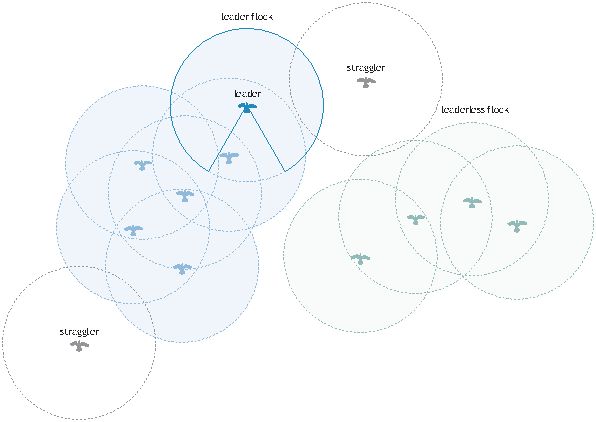
\includegraphics{fig_flock}
  \caption{A leader flock, a leaderless flock and two stragglers. Dashed lines represent the range of potential influence. The shaded areas thus encompass the animats that potentially influence each other and therefore represent the flocks' extents. The solid line in the leader flock represents the visual volume of the leader and shows that even though it potentially influences other members of the flock it is not influenced by any of them.}
  \label{fig:flock}
\end{figure}

With such an interpretation one can distinguish between \emph{flocks} and \emph{stragglers}, where the latter are animats that are not members of any flock. Moreover, by taking into account the perception model used, one can distinguish also between \emph{leader flocks} and \emph{leaderless flocks}. I interpret a leader flock as a flock with at least one \emph{leader} (\ie\ animat that is \sidenote{not}{v1.1.20050210 [FHH]: how about a democratic flock?} influenced by any of its flockmates, but influences at least one), whereas a leaderless flock is a flock with no leader (\ie\ each animat is influenced by at least one of its flockmates).

It should be noted that these definitions represent merely a first-order approximation, but even though they might not be accurate enough from an ornithologist's point of view, they are sufficiently accurate from an algorithmic point of view. It should also be noticed that they in no way suggest or assume the existence of a single and absolute leader, in the sense of a military marching formation. Indeed, as Pomeroy and Heppner \cite{pomeroy:1992} reported, when pigeons make a turn, the birds change position so that a bird at the head of a flock will be in the rear of the flock if the flock turns \ang{180}. Therefore the hypothetical absolute leader would be at the side or rear of the flock after a turn, which means that such a model may not be appropriate at all.

The distinction between leader flocks and leaderless flocks was introduced only to help algorithmic evaluation of the simulated behaviour. Because most real birds have a very good vision to the rear, with the exception of a blind spot directly to the rear, it is very likely that a bird at the head end of a flock will be influenced by trailers. It is thus sound to assume that in nature mostly leaderless flocks exist and if the animats are to display natural looking behaviour, there should be mostly leaderless flocks.

Let the digital universe consist of $n$ animats. Recall from sections~\ref{sec:animat}, \ref{subsec:animat:cwr}, \ref{subsec:animat:fhh}, and \ref{sec:fuzzyAnimat:afd} that in all of the study cases $q_i=\langle \vect{p}_i, \vect{v}_i, s \rangle$ denotes the current state of animat $i$, where $\vect{p}_i \in \E$ and $\vect{v}_i \in \E$ denote the animat's current position in space and velocity, for all $i=1,\ldots,n$. In addition, recall that the current perceivable state of the universe is given as $u=\langle y_1,\ldots,y_n\rangle$ and that the current perceivable data about animat $i$ is $y_i=\lambda(q_i)=\langle\vect{p}_i,\vect{v}_i\rangle$, for all $i=1,\ldots,n$.

Let $\xi_j$ denote the maximal distance between the observed animat and another animat that still allows a `potential direct influence' between them (\ie\ the maximal distance of animat $i$ such that it might still be perceived as relevant by at least one of the perception functions of the observed animat $j$). Then, based on the current perceivable state of the universe $u$, the set $\set{M} \subseteq \set{Y}^n \times \set{Y}^n$, which represents the relation of \emph{potential direct influence} between animats, can be computed
%
\begin{equation}
  \set{M}=\left\{ (j,i)|\ j, i \in \N_n,\ \left\|\vect{p}_i-\vect{p}_j\right\| \leq \xi_j \right\}. \label{eq:metric:M}
\end{equation}

Recall that $r_\textnormal{s}$, $r_\textnormal{a}$ and $r_\textnormal{c}$ denote the separation, alignment and cohesion perception distances of Reynolds's digital bird (definition~\ref{def:animat:s:cwr}). Then, since in Reynolds's case all digital birds are created equal, $\xi_j=\max(r_\textnormal{s},r_\textnormal{a},r_\textnormal{c})$, for all $j \in \N_n$. Similarly, recall that $r_\textnormal{v}$ denotes the visual range of the fuzzy digital bird (definition~\ref{def:fuzzyAnimat:s:afd}) and since in my case all digital birds are also created equal $\xi_j=r_\textnormal{v}$, for all $j \in \N_n$. Therefore the relation of potential direct influence is in fact a set of ordered index pairs $(j,i)$, where animat $i$ is close enough to be treated as relevant by at least one of the perception functions of animat $j$.

Let $g=g_0\ldots g_m$, where $g_i \in \N_n (i=1,\ldots,m)$, denote a series of indexes. The set representing the relation of \emph{potential direct or indirect influence} between animats is then defined as
%
\begin{equation}
  \set{M}^\star= \left\{ (j,k)|\ j, k \in \N_n,\ \exists g \right(g_0=j, g_m=k,\ (g_{i-1}, g_i) \in \set{M}, \forall i \in \N_m\left) \right\}. \label{eq:metric:M*}
\end{equation}

For all $j=1,\ldots,n$ let $\set{G}_j$ denote the set of indexes of animats that potentially directly or indirectly influence animat $j$ or are potentially directly or indirectly influenced by it. Then $\set{G}_j$ is defined as
%
\begin{equation}
  \set{G}_j=\left\{k|\ k \in \N_n,\ \left((j,k) \in \set{M}^\star\ \mathrm{or}\ (k,j) \in \set{M}^\star\right) \right\}. \label{eq:metric:Gi}
\end{equation}

Let a straggler be an animat that is neither potentially directly or indirectly influenced by any other animat nor does it potentially directly or indirectly influence any of them, and let a flock be a set of animats that potentially directly or indirectly influence one or another. Then the set of stragglers is defined as
%
\begin{equation}
  \set{S}=\left\{ \set{G}_j|\ \left|\set{G}_j\right|=1 \right\}, \label{eq:stragglers}
\end{equation}
%
and the set of flocks as
%
\begin{equation}
  \set{F}=\left\{ \set{G}_j|\ \left|\set{G}_j\right|>1 \right\}. \label{eq:metric:flocks}
\end{equation}

As discussed in subsection~\ref{subsec:birdFlocks:fhh}, one of the key questions when studying bird flocks is the existence or necessity of a leader \cite{heppner:1997}. \sidenote{Let a leader be an animat that is a member of a flock but is not directly affected by any of the flock's members.}{v1.1.20050210 [FHH]: biologically not very likely.} In other words, a leader is an animat that is a member of a flock but all of its perception functions find all members of the flock irrelevant. However, since it is a member of the flock, the animat has a potential direct or indirect influence on at least one another member of the flock.

Let $j$ be the index of the observed animat and let the perceived state of the universe be $u$. Then the input of animat $j$ is $x=u$.
As the fuzzy animat is a generalization of the crisp animat (see \chaptername~\ref{ch:fuzzyAnimat}), a crisp perception function (definition~\ref{def:animat:Pi}) can be represented as a fuzzy perception function (definition~\ref{def:fuzzyAnimat:Pi}) and it is safe to assume that the animat's $k$ perception functions return $k$ fuzzy neighbourhoods denoted $\fset{P}_1,\ldots,\fset{P}_k$. Recall that $\fset{P}_i=\langle\fset{N}_i,\fset{O}_i\rangle \in \fpowset{\set{P}^{\mathrm{c}_i}}$, for all $i=1,\ldots,k$. In addition recall that $\fset{N}_i \in \fpowset{\N_n}$ denotes the fuzzy set of indexes of animats that are according to characteristic $\mathrm{c}_i$ relevant to the observed animat. Let $\fset{N}_j$ denote the set $\fset{N}_1 \cup \cdots \cup \fset{N}_k$, then animat $j$ is a leader if and only if $\mu_{\fset{N}_j}(i)=0\ \forall i \in \N_n, i \neq j$ and the set of leader flocks is defined as
%
\begin{equation}
  \set{F}_\textnormal{L}=\left\{ \set{G}|\ \set{G} \in \set{F},\ \exists j \in \set{G}\left(\mu_{\fset{N}_j}(i)=0\ \forall i \in \N_n, i \neq j\right) \right\}. \label{eq:metric:FL}
\end{equation}

\begin{definition}
  \label{def:metrics}
  Let $\set{S}(t)$, $\set{F}(t)$ and $\set{F}_\textnormal{L}(t)$ denote the sets of stragglers, flocks and leader flocks computed from the perceivable state of the universe at the discrete time step $t \in \set{T}$. Then equations~\eqref{eq:metrics0}--\eqref{eq:metrics2} are metrics of the \emph{number of stragglers}, the \emph{number of flocks} and the \emph{proportion of leaderless flocks} at the discrete time step $t \in \set{T}$.
  %
  \begin{equation}
    s(t)=\left|\set{S}(t)\right|, \label{eq:metrics0}
  \end{equation}
  \vspace*{-6mm}
  \begin{equation}
    f(t)=\left|\set{F}(t)\right|,
  \end{equation}
  \vspace*{-2mm}
  \begin{equation}
    f_\ell(t)=1-\frac{\left|\set{F}_\textnormal{L}(t)\right|}{f(t)}. \label{eq:metrics2}
  \end{equation}
\end{definition}

When measuring and judging the flocking behaviour of a group of animats one should first estimate their flocking ability and then the resemblance of their behaviour to that seen in natural flocks. The best choice to estimate the flocking ability is to turn to counting the cumulative number of collisions between animats and to observe the temporal dependency of the number of stragglers and the number of flocks. \sidenote{Since collisions in nature occur rarely, the metrics of cumulative collisions is fairly important and the lower it is, the better the flocking ability.}{v1.1.20050210 [FHH]: but you could have a group -- a swarm -- in which collisions were low, but there would be no coordination -- hence not a flock.} On the other hand, when observing the temporal dependency of the number of flocks the temporal dependency of the proportion of leaderless flocks should always be monitored as well.

A common anomaly when simulating natural phenomena is the lack of similarity to the real thing. For this reason the resemblance of the behaviour of a group of animats should always be compared to that seen in natural flocks. A classical work on the behaviour of flocks and flock formations in general is that of \sidenote{Heppner \cite{heppner:1974a}}{v1.1.20050210 [FHH]: mygoodness! a classical work! I'm flattered.} and thus when estimating the resemblance of the simulated behaviour to that seen in nature, it seems safe to turn to visual inspection of the emerged flocks and their comparison to those presented in Heppner's work (see \chaptername~\ref{ch:birdFlocks}). In addition to that it seems the best option to turn also to observing the temporal dependency of the average nearest neighbour distance and the flight direction and flight speed standard deviations in flocks. Indeed these metrics are the ones that are the most commonly employed by ornithologists \cite{gould:1974,heppner:1985,pomeroy:1992}.

%----
\section{Experiments}
\label{sec:analysis:comparison}
I compared my fuzzy model with Reynolds's through \sidenote{three sets of experiments.}{v1.0.20050124 [MM]: list experiments.} I wanted to estimate the flocking ability of the simulated birds and the resemblance of the displayed behaviour to that seen in natural flocks.

When estimating the flocking ability I turned to counting the number of animat to animat collisions, the dynamics of the number of stragglers, the dynamics of the number of flocks, and the dynamics of the proportion of leaderless flocks.

On the other hand, when estimating the resemblance of the simulated flocks to natural flocks I turned to visual inspection of the emerged flight formations (see \figs~\ref{fig:lineFormations} and \ref{fig:clusterFormations}) as well as the presence of the somewhat erratic, unsystematic behaviour seen in natural flocks \cite{heppner:1990}. \sidenote{I also estimated the level of alignment in flocks by measuring the flight speed and flight direction standard deviations.}{v1.1.20050210 [FHH]: probably a good start.} Furthermore I also observed the degree of uniform distribution by measuring the nearest neighbour distances.

%--
\subsection{Flocking Ability}
In the first set, which consisted of eight experiments, 100 animats were initially placed at random locations having random flight directions and flight speeds.\footnote{Animated versions of the experiments are available in MPEG-4 format on the appended DVD-ROM.} In this set of experiments I was primarily interested if the animats are able to self-organize in flocks. To help self-organization (\ie\ allow animats to eventually meet other animats) I confined the animats using an invisible boundary (see green circle in \fig~\ref{fig:exp:01:01}). Whenever an animat passed this boundary it was forced to turn and eventually return into the confinement without changing its flight speed. In a way this resembles modelling the roosting area used by Heppner  \cite{heppner:1990} (see subsections~\ref{subsec:birdFlocks:fhh} and \ref{subsec:animat:fhh}).

\begin{table*}[!t]
  \footnotesize\renewcommand{\arraystretch}{1}
  \setlength{\tabcolsep}{0pt} % force 0pt intracolumn separation
  \newlength{\halfw}\setlength{\halfw}{.5\linewidth-3.5pt}
  \begin{minipage}[t]{\halfw}
    \begin{tabular}{>{\centering}b{.08\halfw}>{\centering}b{.23\halfw}>{\centering}b{.23\halfw}>{\centering}b{.23\halfw}>{\centering}b{.23\halfw}}
      \toprule
      \multicolumn{5}{c}{Reynold's model} \tabularnewline
      & collisions & stragglers & flocks & proportion of leaderless flocks (avg) \tabularnewline
      \midrule
      01 & 17 & 2 & 2 & 29\pm19 \tabularnewline
      02 & 25 & 2 & 5 & 30\pm17 \tabularnewline
      03 & 14 & 2 & 5 & 29\pm18 \tabularnewline
      04 & 14 & 2 & 5 & 27\pm18 \tabularnewline
      05 & 13 & 0 & 5 & 23\pm19 \tabularnewline
      06 & 10 & 1 & 4 & 31\pm18 \tabularnewline
      07 & 14 & 4 & 6 & 23\pm16 \tabularnewline
      08 & 18 & 7 & 5 & 26\pm16 \tabularnewline
      \midrule
      avg & 15.63\pm4.5 & 2.5\pm2.14 & 4.63\pm1.19 & 26.89\pm17.49 \tabularnewline
      \bottomrule
    \end{tabular}
  \end{minipage}
  \hfill
  \begin{minipage}[t]{\halfw}
    \begin{tabular}{>{\centering}b{.08\halfw}>{\centering}b{.23\halfw}>{\centering}b{.23\halfw}>{\centering}b{.23\halfw}>{\centering}b{.23\halfw}}
      \toprule
      \multicolumn{5}{c}{fuzzy model} \tabularnewline
      & collisions & stragglers & flocks & proportion of leaderless flocks (avg) \tabularnewline
      \midrule
      01 & 0 & 1 & 6 & 83\pm14 \tabularnewline
      02 & 1 & 0 & 3 & 77\pm14 \tabularnewline
      03 & 14 & 0 & 3 & 90\pm12 \tabularnewline
      04 & 0 & 0 & 3 & 80\pm14 \tabularnewline
      05 & 0 & 1 & 5 & 82\pm17 \tabularnewline
      06 & 8 & 0 & 2 & 83\pm17 \tabularnewline
      07 & 0 & 0 & 3 & 77\pm15 \tabularnewline
      08 & 0 & 0 & 6 & 84\pm22 \tabularnewline
      \midrule
      avg & 2.88\pm5.28 & 0.25\pm0.46 & 3.88\pm1.55 & 82.26\pm16.4 \tabularnewline
      \bottomrule
    \end{tabular}
  \end{minipage}
  \caption{A comparison of the number of collisions, number of stragglers and number of flocks after 3000 simulation steps and the overall average proportion of leaderless flocks in the eight experiments used for the estimation of flocking ability for Reynolds's \cite{reynolds:1999} model and my fuzzy model. Note that because in Reynolds's case the area of potential influence is larger, the number of flocks is lower to begin with, so the values cannot be directly compared.}
  \label{tab:exp:01}
\end{table*}

\begin{figure}[p]
  \null\vspace*{1mm}
  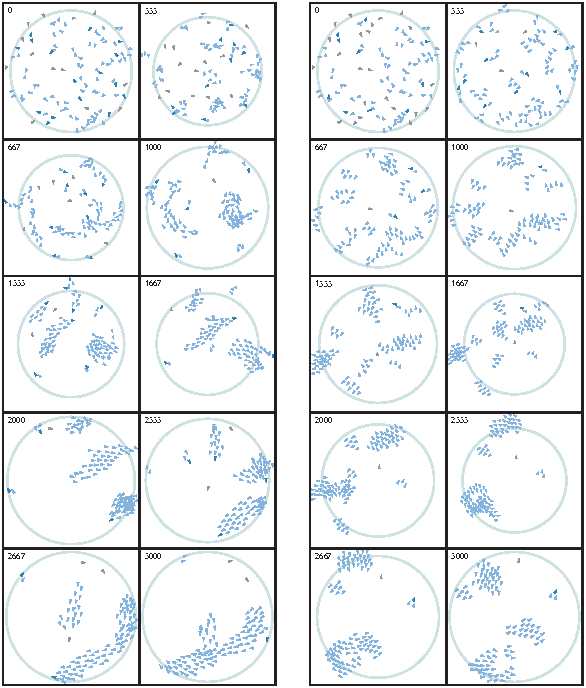
\includegraphics{fig_exp0101}
  \par\vspace*{1mm}
  \caption{A comparison of a series of time-equidistant frames from one of the eight experiments for the estimation of flocking ability for Reynolds's model \cite{reynolds:1999} (left) and my fuzzy model (right). The triangles represent animats, with the apex indicating the flight direction, and the green circle surrounding the animats represents the roosting boundary. Whenever an animat crosses this boundary it is forced to turn and eventually return into the roosting area. For reasons of print clarity the animats' images have been enlarged, which means that their apparent overlapping does not necessarily imply a collision. Furthermore, grey triangles depict stragglers, blue triangles flocking animats and dark blue triangles flock leaders. Orange triangles represent colliding animats.}
  \label{fig:exp:01:01}
\end{figure}
\afterpage{\clearpage}

My animats were strikingly good at avoiding collisions and self-organizing in flocks. While in my case in most cases no collisions occurred, Reynolds's model, summed over the whole population of 100 animats, averaged 15.63\pm4.5 collisions in 3000 simulation steps (see \tab~\ref{tab:exp:01}). In my case I also noticed that, when collisions did occur, they occurred in short periods of time (\eg\ 10 collisions in 200 simulation steps in experiment 03) and were caused by extreme proximity of animats and could be interpreted as side bumping. In Reynolds's case, however, collisions occurred randomly throughout the simulation and were mostly head-on collisions, caused by the merging of flocks.

\begin{figure*}[!t]
  \null\vspace*{2mm}
  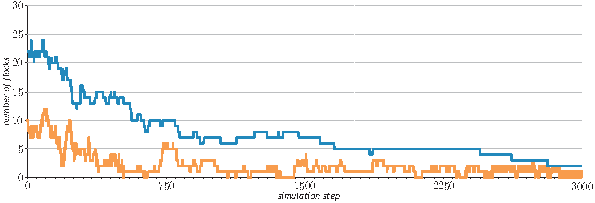
\includegraphics[width=\figurewidth]{chart_exp0101flocks_cwr}
  \par\vspace*{2mm}
  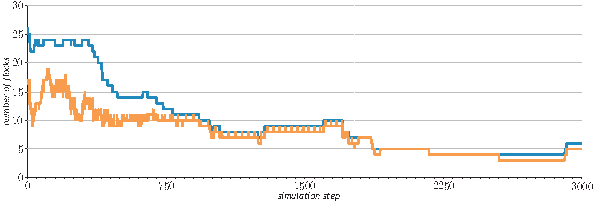
\includegraphics[width=\figurewidth]{chart_exp0101flocks_afd}
  \par\vspace*{2mm}
  \caption{Plot of the number of flocks (blue line) and the contribution of leaderless flocks (orange line) for one of the eight experiments used to estimate the flocking ability of Reynolds's model \cite{reynolds:1999} (top chart) and my fuzzy model (bottom chart). Note that because in Reynolds's case the area of potential influence is larger, the number of flocks is lower to begin with, so the values cannot be directly compared. However, since the number of flocks in both cases decreases through time it can be concluded that the two models present flocking ability. Beside this, it can also be noticed that the fuzzy model produces mostly leaderless flocks whereas Reynolds's model mostly leader flocks.}
  \label{chart:exp:01:01:flocks}
\end{figure*}

Looking at the simulations in real-time I noticed that in my case both classes of flock formations (\ie\ line and cluster formations) emerged, but mostly front cluster ones. Line formations in this set of experiments did not persist for long periods of time. On the other hand, in Reynolds's case the majority of the emerged flocks was of the extended cluster formation whereas line formations did not emerge at all.

Figure~\ref{chart:exp:01:01:flocks} presents a plot of the number of flocks in experiment 01 for my and Reynolds's model. By comparing the proportion of leaderless flocks it can be noticed that in my case mostly leaderless flocks exist, whereas in Reynolds's case mostly leader flocks exist. This tendency was also noticed in the rest of the experiments (see \tab~\ref{tab:exp:01}).

The fact that in Reynolds's model mostly leader flocks emerge is, in my opinion, primarily caused by the perception model used in OpenSteer v0.8 (\ie\ three distinct visual volumes -- one per drive; see subsection~\ref{subsec:animat:cwr}). Not only that the combined perception volume (\figs~\ref{fig:perception:cwr}, \ref{fig:perception:afd} and \ref{fig:perception}) gives the animat a two times larger blind area than my model, it also gives the animat a much larger blind area than the values reported by Heppner \etal\ \cite{heppner:1985}.
%
\begin{figure}
  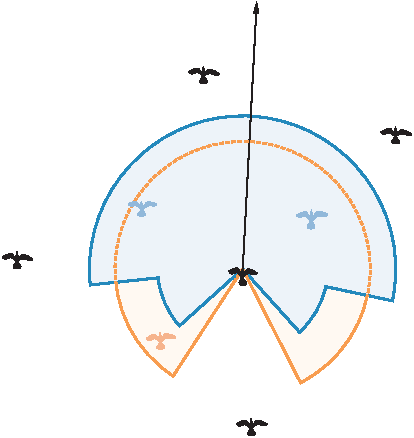
\includegraphics{fig_perception}
  \caption{Comparison of the combined perception volume that Reynolds used in the OpenSteer v0.8 implementation of his model \cite{reynolds:1999} (blue line) and the visual perception volume used in my model (orange line).}
  \label{fig:perception}
\end{figure}
%
As a result it is relatively common that a trailing animat enters the followed animat's blind area and consequently does not influence it any more. The followed animat thus becomes the trailer's leader. Since it is not influenced by any of the flockmates, the leading animat, because no random local disturbances are modelled, keeps its flight speed and flight direction while all of the flockmates only regulate their flight directions and flight speeds to follow it. Therefore, if not confined, the group will eventually form a regularly distributed and stable extended cluster formation (see frames 556--1000 in \fig~\ref{fig:exp:02:14} and 1333--2000 in \fig~\ref{fig:exp:03:01}). According to Heppner \cite{heppner:1974a}, the extended cluster formations in nature may simply be bird aggregations in which birds are flying independently toward a common destination. One might be tempted to conclude that this is precisely what is being experienced here. However, as Heppner states \cite{heppner:1974a}, extended clusters tend to be rather disorganized, with frequent breakoffs and shifts of position, but these features are not to be seen in the leader flocks that emerge from Reynolds's model. This is why I find Reynolds's use of three distinct visual volumes questionable.

%--
\subsection{Cluster Flocks}
In the second set of experiments I was interested if from an initial globular cluster formation, where all animats have the same flight speed and flight direction, natural looking flocks emerge. In this set of experiments no roosting area was modelled. However, I used three initial distribution patterns (see \fig~\ref{fig:exp:02:ini}), for which I changed the nearest neighbour distance (approximately two, four and six body lengths) and initial flight speed (10\%, 50\% and 90\% of maximum flight speed). In other words, there were 27 initial states in all.\footnote{Animated versions of the experiments are available in MPEG-4 format on the appended DVD-ROM.}

\begin{figure}
  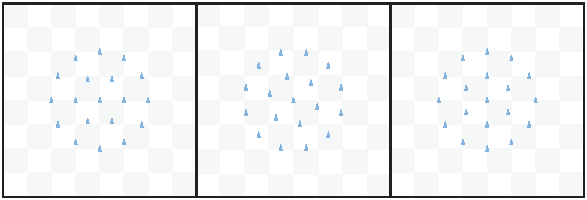
\includegraphics{fig_exp02ini}
  \caption{Initial globular cluster distribution patterns used in the second set of experiments.}
  \label{fig:exp:02:ini}
\end{figure}

Figure~\ref{fig:exp:02:14} presents a comparison of a series of time-equidistant frames from one of the experiments.
%
\begin{figure}[!ht]
  \null\vspace*{1mm}
  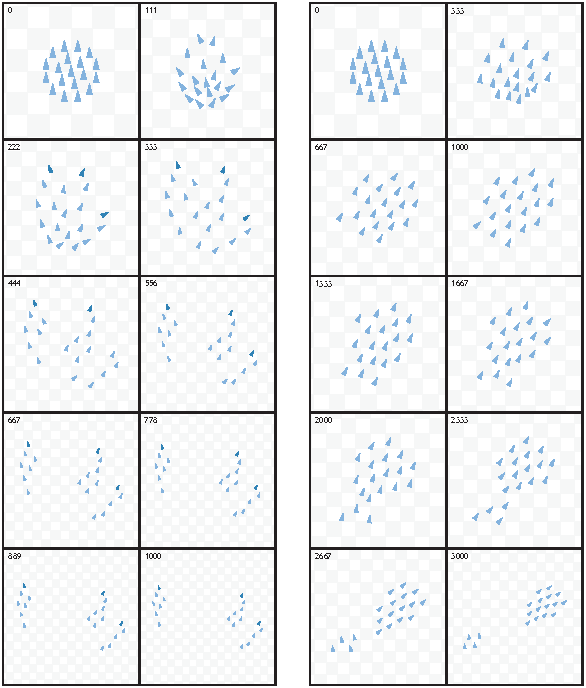
\includegraphics{fig_exp0214}
  \par\vspace*{1mm}
  \caption{A comparison of a series of time-equidistant frames from one of the 27 experiments with a globular cluster initial formation for Reynolds's model \cite{reynolds:1999} (left) and my fuzzy model (right). The triangles represent animats, with the apex indicating the flight direction. The light grey checker board represents a measurement aid with a tile being five body lengths in size. The animats' images have been enlarged for reasons of print clarity and their overlapping does not necessarily represent a collision. Furthermore, blue triangles depict flocking animats and dark blue triangles flock leaders.}
  \label{fig:exp:02:14}
\end{figure}
%
In Reynolds's case in most of the experiments one stable leader flock of the extended cluster formation emerged, which, in the 10000 simulation steps, stabilized flying at exactly maximum speed with the nearest neighbour distance matching the visual range used for the separation drive. The emerged flocks were regularly distributed and highly stable with no position shifting, which is, as already mentioned, the opposite of what can be seen in nature. In the rare cases when position shifting occurred, it originated from the centre of the flock, subsided fast, and the flock stabilized immediately afterwards. The initial flock on average broke off to 1.3\pm0.61 flocks and 0.44\pm1.09 stragglers, with the first breakoff occurring at simulation step 500\pm395.85.

In my case the initial flock on average broke off to 2.33\pm0.83 flocks and no stragglers, with the first breakoff occurring in simulation step 3838.96\pm1680.98. In all cases the animats from the initial flock formation started shifting positions and changing flock formation. The emerged front cluster formations were stable, but when animats, due to position shifting and somewhat erratic and unsystematic behaviour, reorganized into an extended cluster formation, they usually became disorganized and eventually broke off. With breakoffs flock formations from both major classes emerged. The resulting stable cluster flocks were of the front, globular and in few cases even extended cluster formation. The extended cluster formations were disorganized with frequent shifts of position. On the other hand, the resulting stable line flocks were of the `V', echelon and inverted `V' formation. In all cases these flocks were small, consisting of only two or three members and, with the only exception of the inverted `V' formation, they were all leader flocks. The above described behaviour is strikingly similar to natural flocks. If this bears up in future work it will make a very important point. In fact, all previous hypotheses about `V' formation flight assume a functional advantage: aerodynamics \cite{badgerow:1981,badgerow:1988,hainsworth:1987,hainsworth:1989,lissaman:1970}, visibility \cite{heppner:1974a,heppner:1985}, communication \cite{gould:1974,heppner:1974b}, and kinship structure \cite{andersson:2004} (for a review, see \cite{heppner:1997,speakman:1998}). \sidenote{The behaviour present in my experiments seems to suggest instead that even the `V' formation might be an emergent property.}{v1.1.20050210 [FHH]: wow! who would have thought it.}

%--
\subsection{Line Flocks}
In the third set of experiments I was interested if from a front line formation, where all animats have the same flight speed and flight direction, line formation flocks emerge. In this set of experiments no roosting area was modelled. However, I used three initial distributions in which the animats were evenly spaced (approximately two, four and six body lengths) and I changed the initial flight speed (10\%, 50\% and 90\% of maximum flight speed). In other words, there were nine initial states in all.\footnote{Animated versions of the experiments are available in MPEG-4 format on the appended DVD-ROM.}

Figure~\ref{fig:exp:03:01} presents a comparison of a series of time-equidistant frames from one of the experiments.
%
\begin{figure}[!ht]
  \null\vspace*{1mm}
  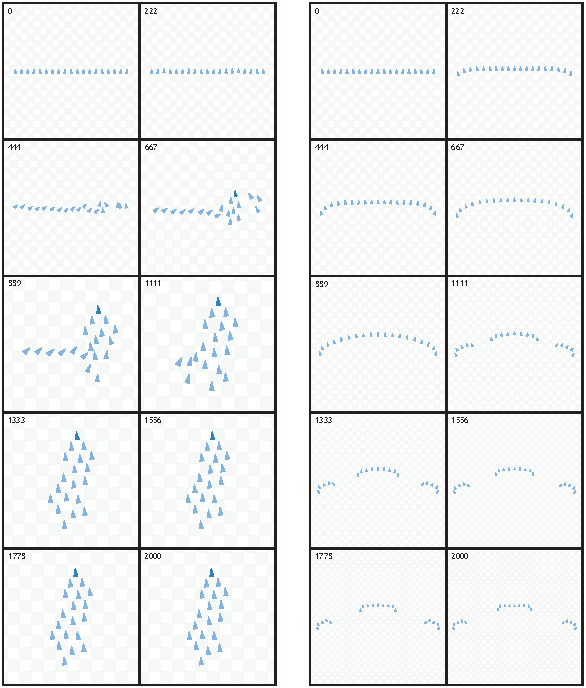
\includegraphics{fig_exp0301}
  \par\vspace*{1mm}
  \caption{A comparison of a series of time-equidistant frames from one of the nine experiments with an initial line formation for Reynolds's model \cite{reynolds:1999} (left) and my fuzzy model (right). The triangles represent animats, with the apex indicating the flight direction. The light grey checker board represents a measurement aid with a tile being five body lengths in size. For reasons of print clarity the animats' images have been enlarged, which means that their apparent overlapping does not necessarily imply a collision. Furthermore, blue triangles depict flocking animats and dark blue triangles flock leaders. Notice that in the fuzzy model the ends of the flock trail away in a curve, which is a very natural behaviour.}
  \label{fig:exp:03:01}
\end{figure}
%
In Reynolds's case the initial flock broke off on average to 1.78\pm1.3 flocks and 1\pm1.8 stragglers and there were 0.33\pm0.5 collisions. Most of the emerged flocks were of the extended cluster formation, regularly distributed and highly stable with no position shifting, but in some rare cases stable, regularly distributed column line formations emerged too. All of the emerged flocks were flying at maximum speed. In my case, on the other hand, the initial flock broke off on average to 3.22\pm0.83 flocks and 1.11\pm1.17 stragglers with no collisions. \sidenote{All of the emerged flocks were of a formation that is similar to the `V' and front line formation -- a \emph{`U'} line formation -- flying at approximately 71\% of maximum speed.}{v1.1.20050210 [FHH]: this is remarkable -- there are aerodynamic reasons for predicting something like this, but this is amazing -- anyway to play with this and get a `V' rather than a `U'?} This behaviour is very surprising. As already stated, all previous hypotheses assume a functional advantege of `V' formation flight (for a review, see \cite{heppner:1997,speakman:1998}), with the most pronounced one being energy saving due to aerodynamic reasons. However, even though the latter is supported both theoretically and empirically \cite{badgerow:1981,badgerow:1988,hainsworth:1987,hainsworth:1989,lissaman:1970,speakman:1998}, it still cannot be supported undisputedly. Mostly because not all large long-distance migrants use formation flight and furthermore because some birds often use acute `V' formations, where the trailing birds, in contrast with the bird at the head of the formation, may make substantial energy savings, while others use more obtuse or bow formations, in which the bird at the head is only a little ahead of its neighbours, and energy savings are probably more equable \cite{andersson:2004}. It is thus impressive that in my experiments, where no aerodynamical aspects as well as no kinship relations \cite{andersson:2004} are taken into account, `U' formations emerge. If by any chance in future work, after the inclusion of a proportion of informed individuals \cite{couzin:2005}, `V' formation flocks will emerge this will represent a remarkable discovery.

